\chapter{Handling Identification}

\section{Exercise 1 - Sine Steer Maneuvers}

\textbf{Q. Perform a set of sine steer maneuvers, with steering wheel angle $\deltd$\ = $\deltdz$\ $\sin(2\pi ft)$. Use $\deltdz$\ = $5^\circ$, and repeat the test at 3 different u = \{50, 80, 100\} km/h.}

        \begin{figure}[ht]
        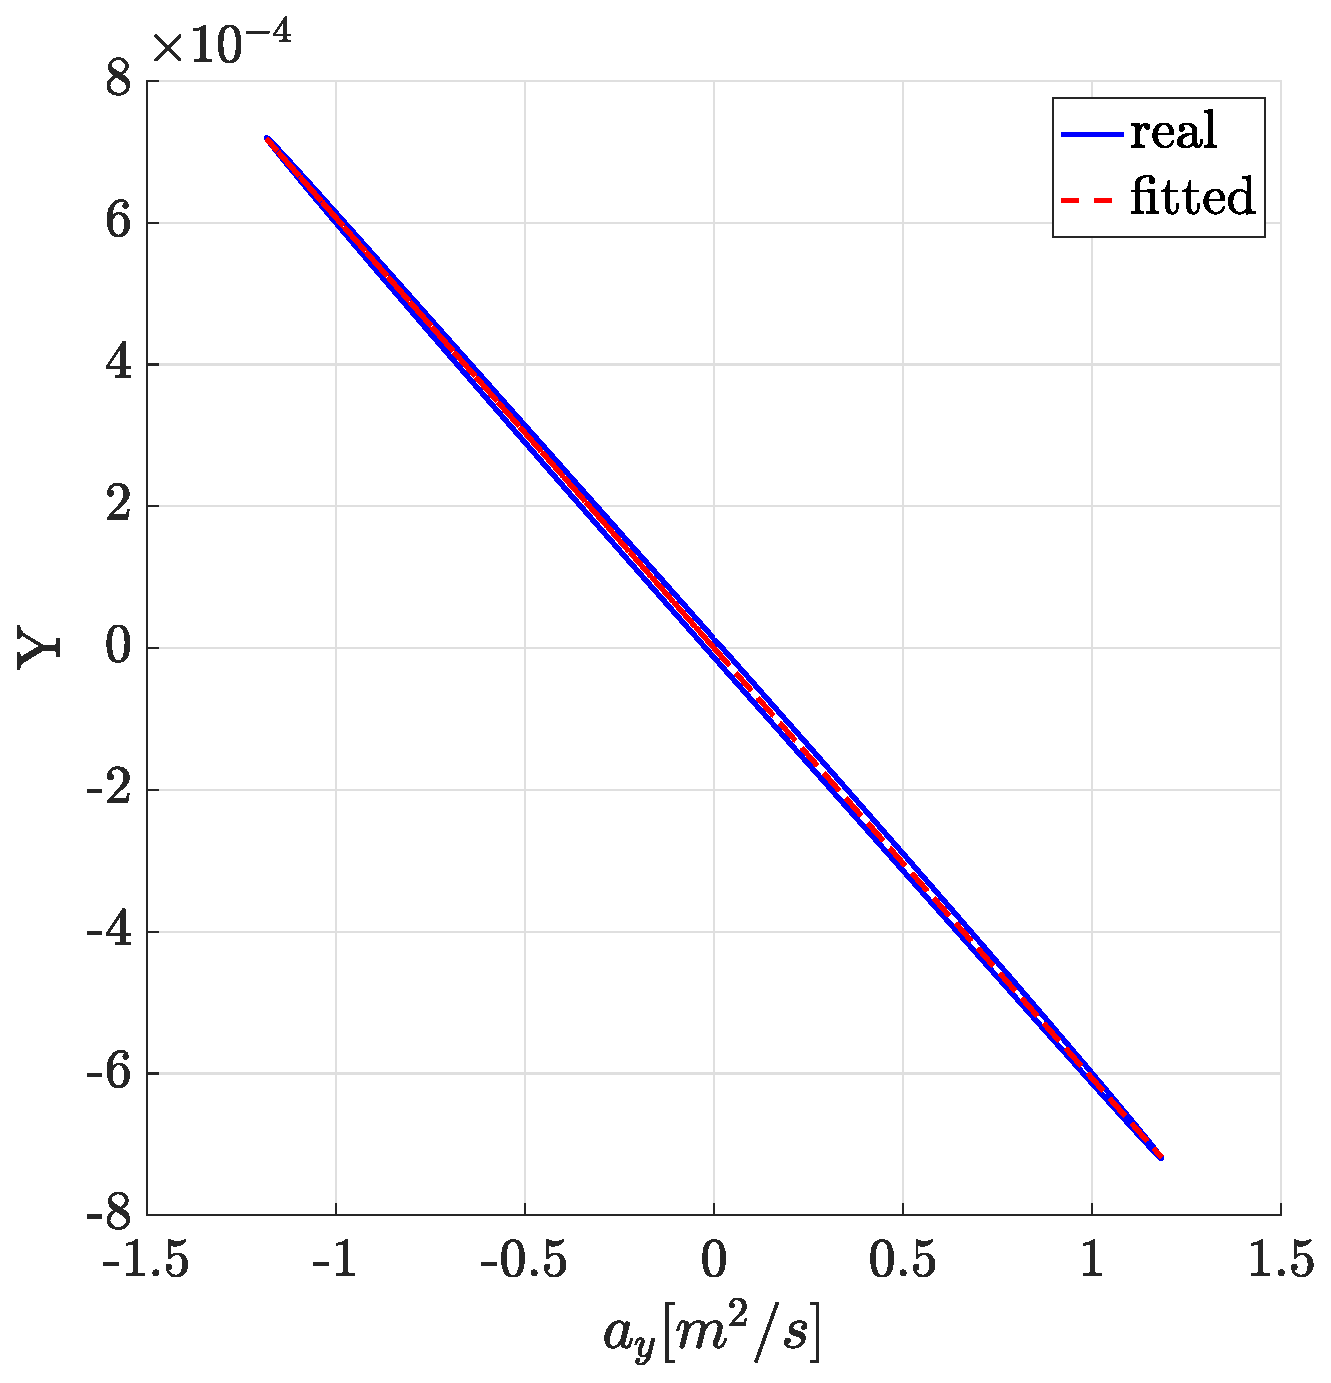
\includegraphics[width=0.5\linewidth]{ex5/q1/ex-51b1.eps}
        \centering
        \caption{Handling diagram result [$\deltdz$\ = $5^\circ$, $u$ = 50 km/h]}
        \label{51b1}
        \end{figure}

Figure \ref{51b1} shows the handling diagram result of a sine steering maneuver that uses a desired steering angle $\deltd$\ = $\deltdz$\ $\sin(2\pi ft)$ at speed 50 km/h. The frequency $f$ in the equation is the number of complete cycles that happen every second. We must perform changes to our system very slowly in order to preserve steady state conditions. The frequency used was $0.001$ $s^{-1}$ and the simulation time was a 1000 s. The  Y refers to the handling behaviour of the vehicle and is calculated using Equation \ref{eq:5.1}:

\begin{equation}\label{eq:5.1}
    Y = \delta - \frac{\Omega}{u} L
\end{equation}

The handling curve obtained at 50 km/h has a negative slope and appears to be linear. The data can be fitted with a first degree polynomial [$f(x) = ax +b$] as shown in Figure \ref{51b1}.

The negative slope indicates that the vehicle exhibits an over-steering behaviour. Over-steering occurs when the vehicle's rear wheels have higher lateral slip compared to the front [$\alpha_{r} > \alpha_{f}$]. This causes the rear wheels to have a larger radius of curvature than the front and the vehicle steers more than expected. If we want to keep the same radius of curvature in an over-steering condition, we must decrease the steering angle $\delta$ at higher velocities.

        \begin{figure}[ht]
        \includegraphics[width=0.99\linewidth]{ex5/q1/ex-51c.eps}
        \centering
        \caption{Handling diagram results at different speeds}
        \label{51c}
        \end{figure}

The slope of the line represents the under-steering gradient $\kus$. It describes the evolution of $\delta$ as $\ay$ increases. $\kus$ is positive if the vehicle is under-steering and negative when over-steering.

Increasing the speeds to 80 and 100 km/h resulted in an increase in the lateral acceleration $\ay$ as shown in Figure \ref{51c}. The vehicle nonetheless showed over-steering behaviour across all the simulated speeds. A comparison between the yaw-rate $\Omega$ and the desired steering angle $\deltd$ shows that the $\Omega$ keeps increasing with higher speeds while $\deltd$ does not.

        \begin{figure}[ht]
        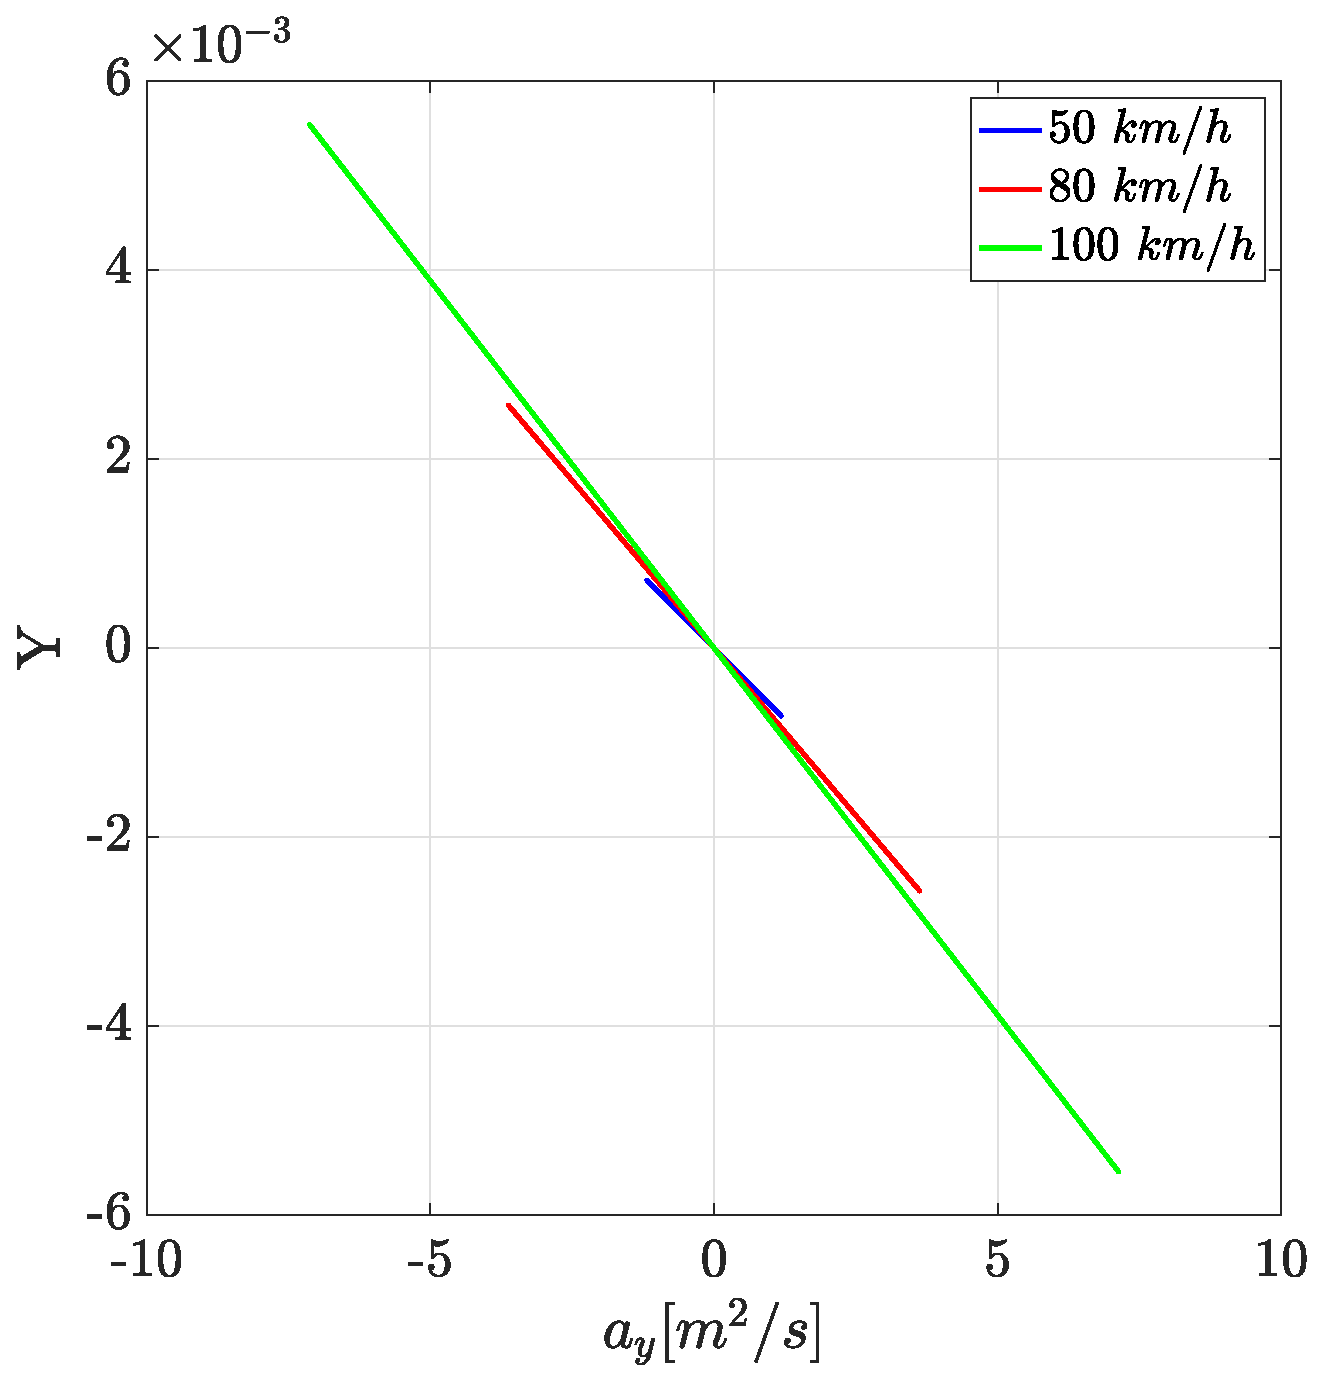
\includegraphics[width=0.6\linewidth]{ex5/q1/ex-51d.eps}
        \centering
        \caption{Handling curve comparison}
        \label{51d}
        \end{figure}
        
Superimposing the handling curves of the three simulated speeds in Figure \ref{51d} clearly shows that with higher speeds, the over-steering behavior increases [steeper negative slope]. That means $\delta$ will need to be decreased even further with higher speeds to keep the same curvature. Furthermore, the obtained curves pass through the origin. That means when there is no lateral acceleration $\ay$, the steering behaviour will be neutral. 

        \begin{figure}[ht]
        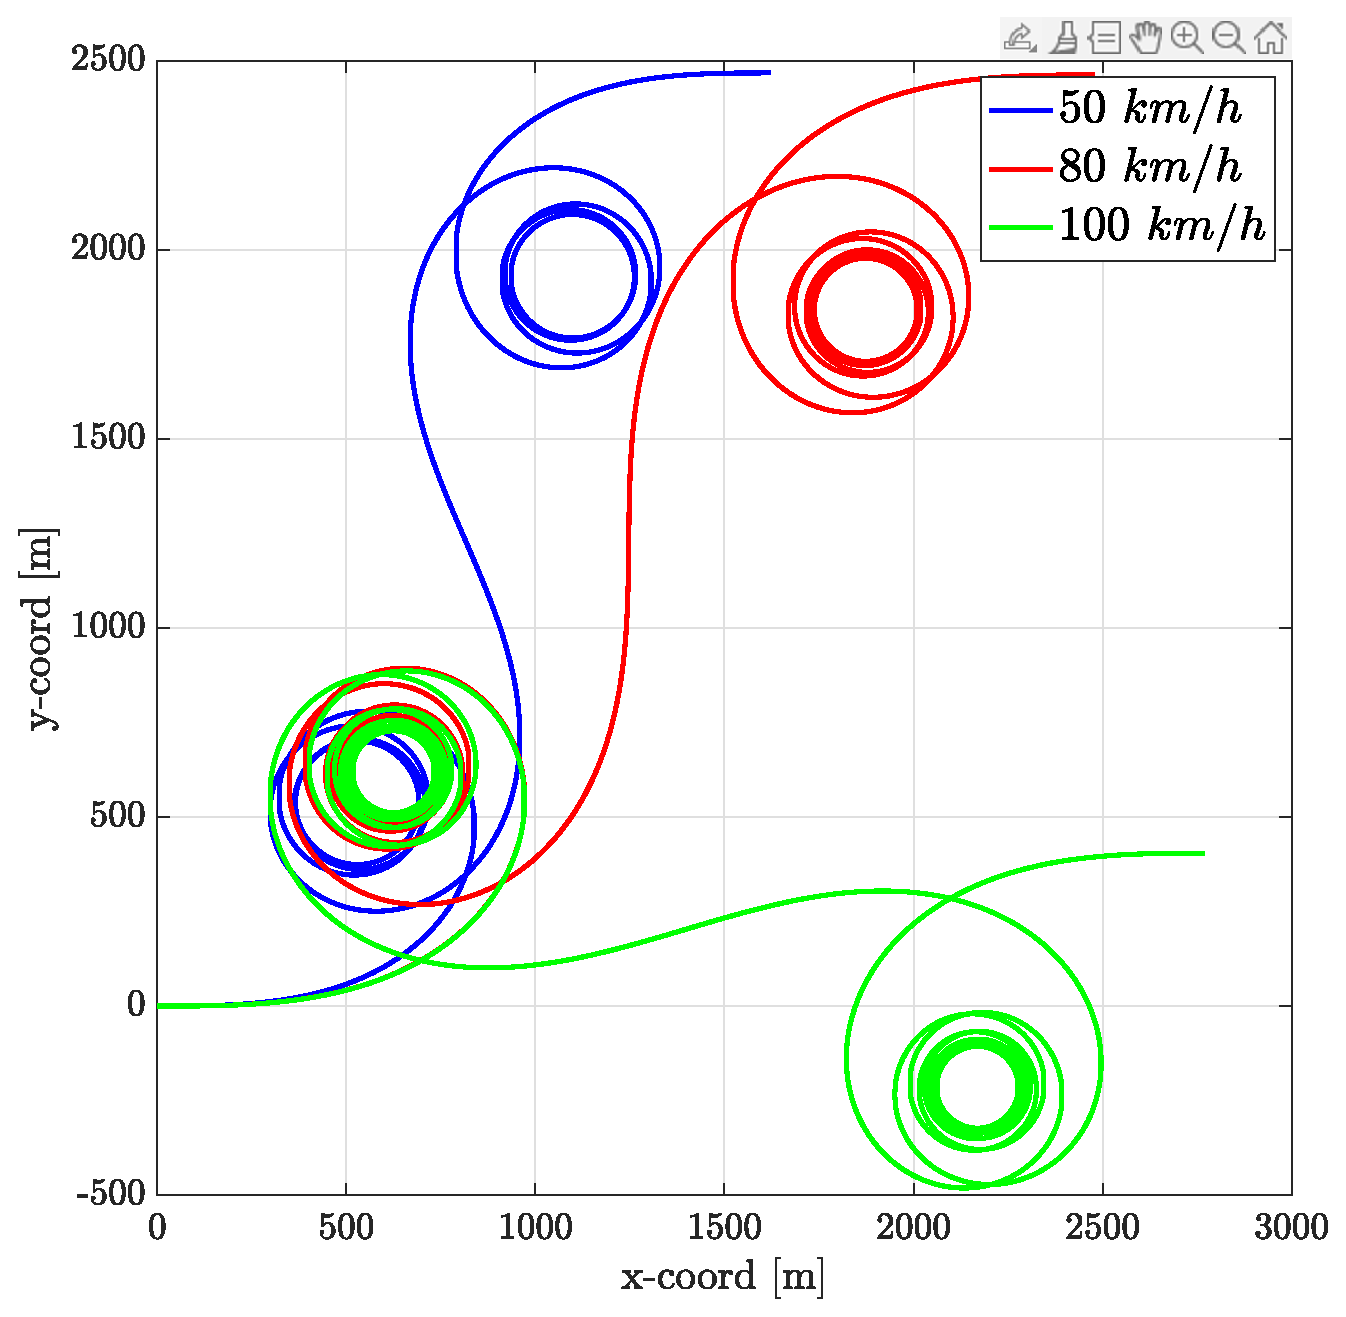
\includegraphics[width=0.6\linewidth]{ex5/q1/ex-51a.eps}
        \centering
        \caption{Vehicle paths for sine steer maneuvers at different speeds}
        \label{51a}
        \end{figure}
        
Plotting the path results of the three different speeds, as shown in Figure \ref{51a}, confirms the over-steering behaviour. The radius of the curvature [the size of the circles] decreases with increasing velocities.

\textbf{Q. carry out other 3 sine steer maneuvers, with these data: \vspace{-1em}
\begin{enumerate}
    \item \boldmath$\deltdz$ = $70^\circ$ , $u$ = 50 km/h
    \item $\deltdz$ = $24^\circ$ , $u$ = 80 km/h
    \item $\deltdz$ = $12^\circ$ , $u$ = 100 km/h
\end{enumerate}}

\section{Exercise 2 - Constant Steer Maneuvers}
